\documentclass[journal,twocolumn]{IEEEtran}


%
\ifCLASSINFOpdf

\else

\fi


\usepackage{amsmath} % математическая мода
\usepackage{amssymb} % математическая мода

\usepackage{graphicx}
\usepackage[ruled,vlined]{algorithm2e}


\newcommand{\dint} {\displaystyle\int}
\newcommand{\dsum} {\displaystyle\sum}
\newcommand{\dprod} {\displaystyle\prod}

\newtheorem{theorem}{Theorem}
\newtheorem{remark}{Remark}
\newtheorem{lemma}{Lemma}
\newtheorem{proposition}{Proposition}
\newtheorem{assumption}{Assumption}
\newtheorem{definition}{Definition}


\newcommand{\co}{\operatorname{co}}




\hyphenation{op-tical net-works semi-conduc-tor}


\begin{document}
%
% paper title
% Titles are generally capitalized except for words such as a, an, and, as,
% at, but, by, for, in, nor, of, on, or, the, to and up, which are usually
% not capitalized unless they are the first or last word of the title.
% Linebreaks \\ can be used within to get better formatting as desired.
% Do not put math or special symbols in the title.
\title{Flight simulator based on robotic arm with acceleration tracking under restricted position  non-convex working space}

\author{Viktor Chertopolokhov, Olga Andrianova, Alejandra Hernandez-Sanchez, Caridad Mireles
        and Isaac Chairez% <-this % stops a space
\thanks{M. Shell was with the Department
of Electrical and Computer Engineering, Georgia Institute of Technology, Atlanta,
GA, 30332 USA e-mail: (see http://www.michaelshell.org/contact.html).}% <-this % stops a space
\thanks{J. Doe and J. Doe are with Anonymous University.}% <-this % stops a space
\thanks{Manuscript received April 19, 2005; revised August 26, 2015.}}



\markboth{Journal of \LaTeX\ Class Files,~Vol.~14, No.~8, August~2015}%
{Shell \MakeLowercase{\textit{et al.}}: Bare Demo of IEEEtran.cls for IEEE Journals}



% make the title area
\maketitle

\begin{abstract}
This study aims to design a state feedback controller of a multiarticulated robotic arm operating as a flight simulator operating on a restricted working space. 
\end{abstract}

\begin{IEEEkeywords}
Flight simulator; Robotic arm; Dynamic imitation; Restricted working space; Acceleration tracking.
\end{IEEEkeywords}



\IEEEpeerreviewmaketitle



\section{Introduction}

\IEEEPARstart{F}{light} simulators are complex electromechanical systems that can reproduce the .


All motion simulators have the aim of reproducing the sensation of being on an actual mobile device evolving on a a simulation environment. The achievement of this goal implies that the user may feel sensory inputs as close to real as possible. Most of the motion simulators try to induce the sensation using vision and hearing mainly, however it has been proven that motion cues are needed if the immersion is expected.

Motion (flight, driving and so many others) simulators are actually in wide spread application for a multitude of purposes. Safeness, cheapness, flexibility and easily controllability surrounding to train users (including both civilian and military pilots) are motivating characteristics for developing motion simulators. These simulators can be also used in both, normal operation and the handling of extreme situations, which could not be performed safely in a real world setting.

In addition, they are common tools for medical and biomedical researchers to evaluate how induced accelerations as well as angular velocities are sensed by pilots under training, for testing new vehicles designs and some more applications. 



XXXXXXXXXXXXXXXXXXXX

XXXXXXXXXXXXXXXXXXXX



\section{Problem statement}

This study considers the design of an automatic controller that may reproduce the requested positions 

The application of the well-known direct kinematics technique yields to calculate the three-dimensional coordinates of the robotic end-effector $p \in \mathbb{R}<{3}$ which is functionally connected to the joint-configuration $q$ by a nonlinear vector function $H : \mathbb{R}<{3} \rightarrow \mathbb{R}<{n} $, that 
%
\begin{equation}
    p =H(q) 
\end{equation}

The dynamic motion of the suggested robotic arm may be described as follows:
%
\begin{equation}
    \begin{array}{c}
         M\left( q \right) \dfrac{d^2 }{d t^2} q+  C\left( \dfrac{d }{d t} q , q \right) \dfrac{d }{d t} q + G(q) = \tau + \dsum_{i = 1}^{p} \lambda^{\top}_{i} A_{i} \left( q \right)     \end{array}
         \label{DynamicModel}
\end{equation}

The vector $q \in \mathbb{R}^{n} $ defines the set of joints variations (either prismatic or revolute) in the FSRA, while the vector $\tau \in \mathbb{R}^{n}$ defines the set of generalized forces affecting the flight simulator.   

The expression given in \eqref{DynamicModel} describes the dynamics of 
the robotic arm with $M: \mathbb{R}^{n} \rightarrow \mathbb{R}^{n \times n}$ the inertia matrix, $C: \mathbb{R}^{n} \times \mathbb{R}^{n} \rightarrow \mathbb{R}^{n \times n}$ the Coriolis matrix and $G : \mathbb{R}^{n} \rightarrow \mathbb{R}^{n}$ the vector that characterizes the gravitational effects over the arm. 

An efficient flight simulator must provide not only a correct positioning of the end effector associated to the robotic arm, but a tracking of the acceleration (translational and rotational) that compensates the overload detected at the pilot's head by the otholitic system. 


Defining the extended reference state vector $P^{*}= \left[ \left(p^{*}\right)^{\top},\left(\dfrac{d }{d t} p^{*} \right)^{\top}, \left( \dfrac{d^{2} }{d t^{2}} p^{*} \right)^{\top} \right]^{\top}$, the problem associated to the control design can be be formulated as to propose an automatic controller such as the following inequality holds
%
\begin{equation}
    \begin{array}{c}
         \left\Vert P(t) - P^{*}(t) \right\Vert \leq \beta  
    \end{array}
    \label{TrackingProblemEndEffector}
\end{equation}

\noindent where $ P= \left[ p^{\top},\dfrac{d }{d t} p^{\top}, \dfrac{d^{2} }{d t^{2}} p^{\top} \right]^{\top}$ defines the extended state corresponding the movement of the RAFS. The constant $\beta$ characterizes the quality of tracking for the extended state that includes position, velocity and acceleration tracking. 

The tracking problem \eqref{TrackingProblemEndEffector} must be solved considering that the configuration of the robotic arm defines a restricted workspace $\Omega=\Omega(q)$. This is a significant characteristic of this motion simulator since such restrictive workspace may limit the continued motion during the flight simulation task. 

The existence of the direct kinematics justifies the existence of a feasible inverse function $H^{-1}$, that is $q := H^{-1}(p)$, which corresponds the inverse kinematics. This inverse solution allows to estimate $ \dfrac{d}{dt} q $ and $ \dfrac{d^{2}}{dt^{2}} q$. Then, the corresponding extended vector  for the articulations can be proposed $Q = \left[ q^{\top},\dfrac{d }{d t} q^{\top}, \dfrac{d^{2} }{d t^{2}} q^{\top} \right]^{\top}$. Then, the motion problem for the RAFS can be restructured as: To design a control $\tau$ such that the joint trajectory tracking defined as
%
\begin{equation}
    \begin{array}{c}
         \left\Vert Q(t) - Q^{*}(t) \right\Vert \leq \beta_{Q}  
    \end{array}
\end{equation}

\noindent with $Q^{*} = \left[ (q^{*})^{\top},\dfrac{d }{d t} (q^{*})^{\top}, \dfrac{d^{2} }{d t^{2}} (q^{*})^{\top} \right]^{\top}$ , the corresponding extended state reference vector and $\beta_{Q}$ the positive scalar that defines the quality of tracking in the joint space. Once more, the joint restrictions corresponding the admissible workspace must be taken into account. 



\section{The robotic arm flight simulator}

Nowadays, there is a general trend to take advantage of movement abilities of robotic manipulators to create effective flight simulators that imitate pilot sensations along actual flying experience. The implementation of such robotic arms requires having a combination of slower and faster movements that may induce the observed combined movements in flight simulators. 


This study considers a particular robotic arm made of N rotational articulations that can move over a three dimensional space. The robotic configuration includes a traditional robotic arm of N-2 degrees of freedom and an end effector made of two additional rotative joints.

\begin{figure*}
    \centering
    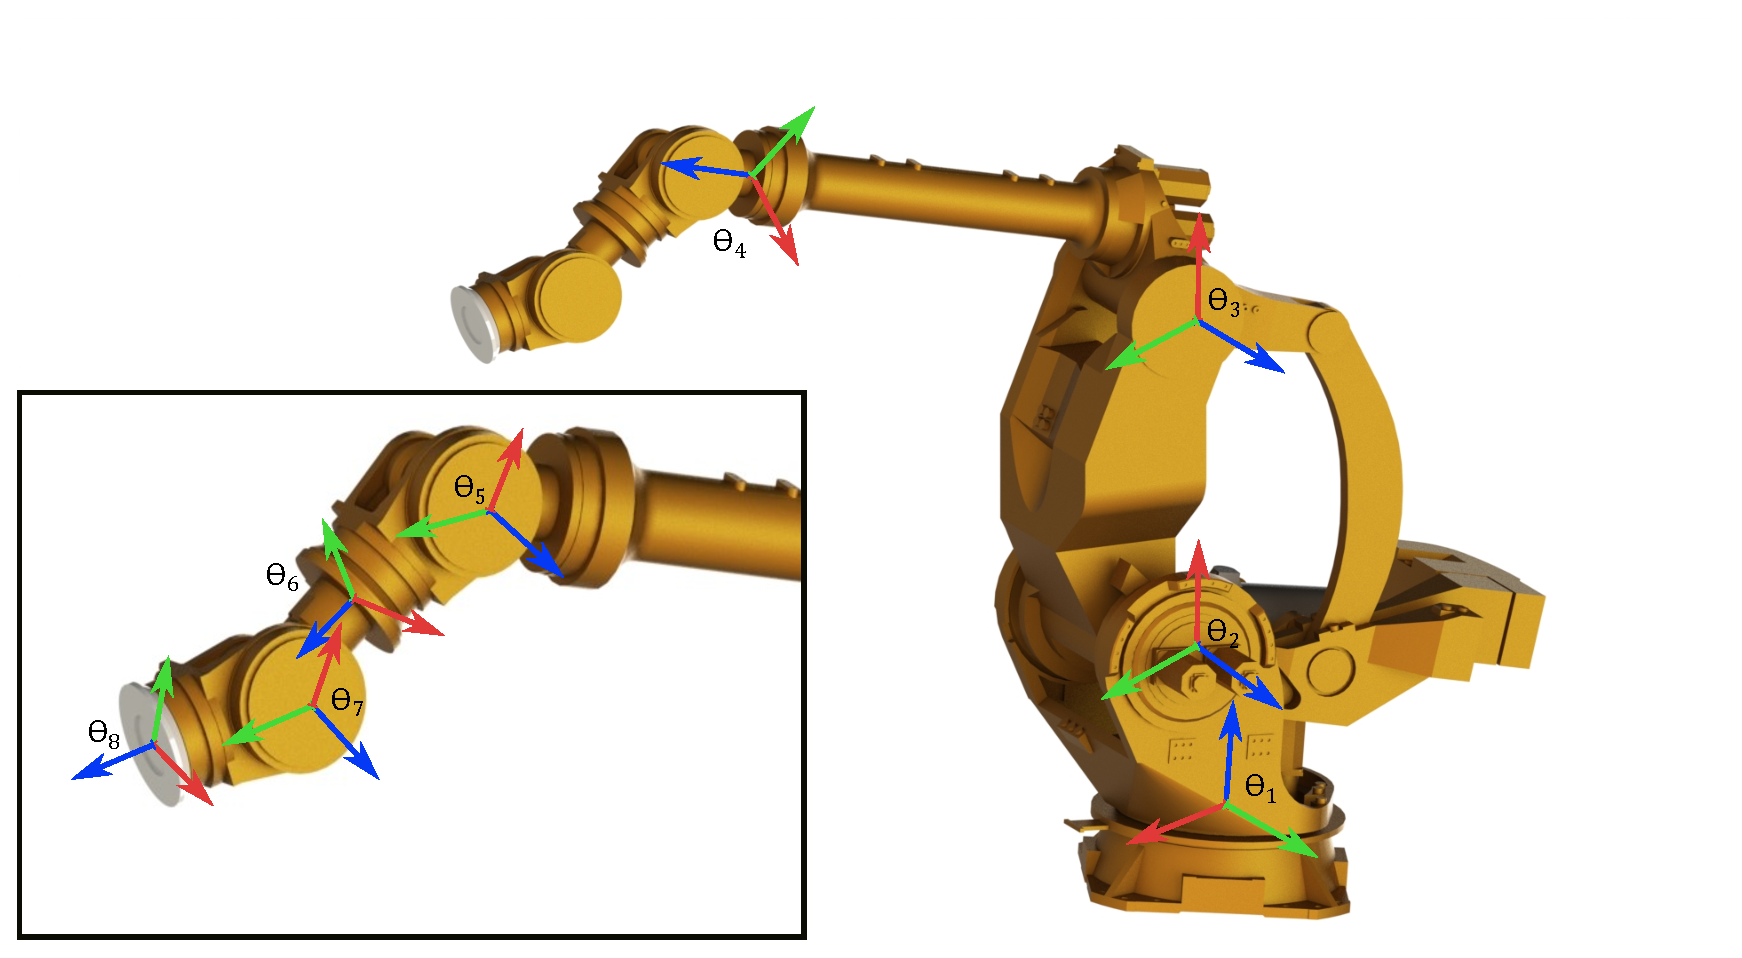
\includegraphics[scale=0.6]{Figures/RoboticArm.eps}
    \caption{Caption}
    \label{fig:RoboticArmConf}
\end{figure*}



The configuration of the proposed robotic arm and its corresponding mathematical model can be represented as as follows 

\begin{equation}
\begin{array}{c}
\dot{x}_{a}=x_{b} \\ 
\dot{x}_{b}= F \left( x_{a},x_{b}\right) +G\left( x_{a}\right) u + \xi\left( x_{a},x_{b},t\right)%
\end{array}%
\label{StateVar}
\end{equation}%

Here $x_{a} = q $ and $x_{b} = \dot{q} $. The function $F: \mathbb{R}^{n} \times \mathbb{R}^{n} \rightarrow \mathbb{R}^{n}$ is known as the drift and collects the Coriolis and gravitational elements. The function $G : \mathbb{R}^{n} \rightarrow \mathbb{R}^{n \times n}$ defines the effect of the input to the dynamics of the RAFS. The term $\xi : \mathbb{R}^{n} \times \mathbb{R}^{n} \times \mathbb{R}^{+} \rightarrow \mathbb{R}^{n }$ defines the gathered effect of external perturbations and modeling imprecision. 

The functions included in \eqref{StateVar} satisfy the following assumptions:

\begin{assumption}
The drift term $F$ admits the following inequality:
%
\begin{equation}
    \left\Vert F \left( x_{a},x_{b}\right) \right\Vert \leq f_0 + f_1 \left\Vert x \right\Vert + f_2 \left\Vert x \right\Vert^{2}
\end{equation}
 
\noindent where $f_0$, $f_1$ and $f_2$ are positive constants and $x = \left[ x^{\top}_{a}, x_{b} \right]^{\top}$. The presence of these three terms is justified considering the inclusion of frictions forces, gravitational effect and Coriolis terms. 
\end{assumption}

In order to keep the controllability of the system \eqref{StateVar}, the following assumption holds in this study:

\begin{assumption}
Matrix $G\left( x_{a}\right)$ has a no null determinant for all admissible $x_{a}$.
\end{assumption}

The perturbed dynamics of the robotic arm requires that $\xi\left( x_{a},x_{b},t\right)$ is not only integrable, but belongs to the following admisslbe set:

\begin{assumption}
    The admissible set of external perturbations and internal modelling uncertainties is given by:
    %
    \begin{equation}
        \Xi_{adm} = \left\lbrace \xi \in \mathbb{R}^{n} \mid \left\Vert \xi \right\Vert \leq  \xi_{0} + \xi_{1} \left\Vert x \right\Vert + \xi_{2} \left\Vert x \right\Vert^{2} \right\rbrace
    \end{equation}
    with $\xi_0$, $\xi_1$ and $\xi_2$ positive constants. The vector $\xi$ is differentiable with respect to time with the derivative satisfying
    %
    \begin{equation}
         \left\Vert \dfrac{d}{dt} \xi \right\Vert \leq  d\xi_{0} + d\xi_{1} \left\Vert x \right\Vert + d\xi_{2} \left\Vert x \right\Vert^{2}
    \end{equation}
    with $d\xi_0$, $d\xi_1$ and $d\xi_2$ positive constants.
\end{assumption}

Assumption 3 holds considering the same arguments introduced for the nonlinear function $F$.

\section{End-effector working space}


Robotic arm based flight simulators have significant advantages with respect to alternative configurations using parallel robotic devices (such as Stewart platform) or free rotational structures. Nevertheless, there is an accepted idea regarding the robotic arm based configuration has the disadvantage of having restricted working space that may limit the quality of dynamic imitation enforced by the simulator. The restricted robotic workspace can be estimated considering the direct kinematics of the arm configuration. In the specific case of using robotic arm as the mechanical basis of the flight simulator, the efficient estimation of the workspace has a relevant implication on the path trajectory that must be traced by the end-effector of the FSRA. 
%to be reconsidered according to FANUC numeration

\begin{figure}[!h]
    \centering
    \begin{subfigure}{0.2\textwidth}
        \includegraphics[width = \linewidth]{Figures/mathmodel.png}
        \caption{Arm configuration in vertical plane}
        \label{fig:mathModelVert}
    \end{subfigure}
    \begin{subfigure}{0.35\textwidth}
        \includegraphics[width = \linewidth]{Figures/posSet.jpg}
        \caption{The adm set}
        \label{fig:posVert}
    \end{subfigure}
    \caption{}
\end{figure}

As a simplified approximation, the linear position of the cabin could be characterized by several parameters: $\varphi$ ~ --- the angle of deviation of the main link from the vertical axis, $\alpha$ ~ --- the angle of deflection of the second vertical-plane link relative to the main, $l_1$ and $l_2$ ~ --- the lengths of the links, respectively.

During the movement of the stand in the vertical plane, the coordinates of the end point of the stand satisfy the following relations:
\begin{equation}
    \begin{cases}
        x = l_1\sin\varphi + l_2\sin(\phi + \alpha),
        \\
        y = l_1\cos\varphi + l_2\cos(\phi + \alpha),
    \end{cases}
    \label{eq:point_coords}
\end{equation}

The set of admissible geometric positions $P$ of cabin in the vertical plane could be easily drawn. The contour of the set $ P $ consists of arcs of several circles. The radius of the larger arc centered at $ O_1 $ is $ r = l_1 + l_2 $, and the radius of the smaller $ \rho $ can be found using the following formula:
\begin{equation}
    \rho = \sqrt{l_1^2 + l_2^2 + 2 l_1 l_2 \cos\alpha_{\max}}.
\end{equation}

The set $ P $ has an asymmetric form. To solve the problem of dynamic simulation, it is desirable to have such an area in which it is possible to move with maximum acceleration equally in all directions from a certain starting position. In the set $ P $ one can inscribe a family of circles of radius $ R = l_1 + l_2 - \rho $, the collection of centers of which makes up the arc $ AB $. The circles themselves form the region $ D $, which lies in $ P $. Let's call the arc $ AB $ as a starting arc. The coordinates $ a $ and $ b $ of the arc $ AB $ can be written as:
\begin{equation}
    (a,b)=\{(R+\rho)\sin\beta, (R+\rho)\cos\beta\}
    \label{eq:circle}
\end{equation}
where $\beta\in[\beta_{\min},\beta_{\max}]$, and $\beta_{\min}$, $\beta_{\max}$ should be defined. 

Consider in fig. \ref{fig:posVert} triangle $ O_1O_2A $: $ O_1O_2 = l_1 $, $ O_1A = \rho + R $, $ O_2A = l_2 + R $. $ O_2M = l_2 $ and $ MA = R $ ($ O_2M $ and $ MA $ as
the radii are perpendicular to the tangent to the corresponding circles at the point M and form a segment $ O_2A $). By the cosine theorem:
\begin{equation*}
    \cos(\angle O_2O_1A)=\cos(\varphi_{\min}+\beta_{\min})=
    \frac{l_1^2+(\rho+R)^2-(l_2+R)^2}{2l_1(\rho+R)}
\end{equation*}

\begin{equation}
    \beta_{\min}=\arccos\frac{\rho^2+l_1^2-l_2^2+2R(\rho-l_2)}{2l_1(\rho+R)}-\varphi_{\min}
\end{equation}

Let us prove that $ \beta _ {\max} = \varphi _ {\max} $. The lower arc of the set $ P $ centered at $ O_2'$ has radius $ l_2 $. A circle centered at $ B $ has a radius $ R $ that satisfies the relation $ 2R> l_2 $. If $ \beta> \varphi _ {\max} $, then the points of the circle with center $ B $ and radius $ R $ will go beyond the set $ P $.

Thus, an area $ D $ for the end point of the manipulator is obtained, in which the process of dynamic simulation can be carried out.

Here $ P $ is the set of all admissible positions of the point $ M $, $ D $ is a figure within which further movement will be carried out in the process of dynamic simulation, $ \breve {AB} $ --- The `` starting '' arc from which we will start and where we will end the simulation process. The arc radius $ \breve {AB} $ is $ \rho + R $. $ R $ --- the radius of the largest circle that is entirely in $ D $ and whose center is $ \in \breve {AB} $. $ \rho $ ~ --- radius of the arc forming the left boundary of $ D $. $ R $ and $ \rho $ depend on the parameters of the robot-manipulator and can be found by the formulas:
\begin{equation*}
    \rho = \sqrt{l_1^2+l_2^2+2l_1l_2\cos\alpha_{\max}},
\end{equation*}
\begin{equation*}
    R = l_1 + l_2 - \rho,
\end{equation*}
where $\alpha_{\max}$ ~--- the maximum of $\alpha$.
 $\beta_{\min}$ and $\beta_{\max}$ can be found by the formulas:
\begin{equation*}
    \beta_{\min} = \arccos\frac{\rho^2+l_1^2-l_2^2+2R(\rho-l_2)}{2l_1(\rho+R)}-\varphi_{\min};\ \
    \beta_{\max} = \varphi_{\max},
\end{equation*}
where $\varphi_{\min}$ and $\varphi_{\max}$ are minimum and maximum for $\varphi$.

Thus, a working space for the cabin has been obtained for the simplified 2-chain approximation.

The specific estimation of the workspace depends on the mechanical configuration of the motion simulator. There is not a general formalism to estimate the FSRA. In recent years, extensive evaluation of the direct kinematics, application of MonteCarlo simulations, genetic algorithms, neural networks and so many others. 

This study considers the mechanical configuration of a FANUC M-2000iA-900L multi-articulated robotic arm to design the RAFS. An extensive study of the direct kinematics considering the joints limited angular ranges (Table \ref{tab:TableAngMov}) served to characterize the admissible (no-convex) workspace. 
%
\begin{table}[!h]
    \centering
    \caption{Ranges of angles in the FANUC M-2000iA-900L}
    \begin{tabular}{c|c|c}
         Angle & Minimal Value & Maximal Value \\
         \hline
         \hline 
         $q_{1}$ & $-165 ^{o}$ & $165 ^{o}$ \\
         $q_{2}$ & $-80 ^{o}$ & $80 ^{o}$ \\
         $q_{3}$ & $-82.5 ^{o}$ & $82.5 ^{o}$ \\
         $q_{4}$ & $-360 ^{o}$ & $360 ^{o}$ \\
         $q_{5}$ & $-120 ^{o}$ & $120 ^{o}$ \\
         $q_{6}$ & $-360 ^{o}$ & $360 ^{o}$ \\
         $q_{7}$ & $-120 ^{o}$ & $120 ^{o}$ \\
         $q_{8}$ & $-360 ^{o}$ & $360 ^{o}$ \\
         \hline
         \hline
    \end{tabular}
    \label{tab:TableAngMov}
\end{table}

The technique proposed in \cite{SSS} leads to estimate the admissible workspace of the proposed RAFS (Figure \ref{f:Workspace}). 

\begin{figure*}
    \centering
    \includegraphics[scale=0.3]{Figures/Rango.JPG}
    \caption{Admissible workspace of the developed RAFS.}
    \label{fig:RoboticArmConf}
\end{figure*}

Usually, the estimated workspace of the robotic arm (such as in this study) is not convex which may difficult the design of an automatic controller that can solve the tracking trajectory problem presented in \eqref{ProbState}. This fact motivates the inclusion of a preliminary procedure to design an inner convex cover for the estimated non-convex workspace. 

The estimation of the inner convex region that is further considered into the automatic controller design with position constraints, that enforces the existence of velocity and acceleration restrictions as well considering the RAFS device configuration (including the kind of actuators included in it).  




%The algorithm used in this study considered the successive application of the  L\"owner-John to calculate inner Ellipsoids of restrictive regions delimited by a polytope. 

The mentioned polytope was derived considering the non-convex workspace of the RAFS. To do so, a set of $N_r, (N_r \geq 4)$ three-dimensional coordinates was proposed within the non-convex admissible workspace. These points appear in Figure \ref{f:xxx} marked with a diamond. Notice that depending on the number of such markers the number of developed state limitations can vary. 

Noticing the RAFS working space, the non-convex admissible workspace can be represented with a semi-algebraic set (associated to some polynomials) $ S= \left\lbrace p \in \mathbb{R}^{3} \mid p_{i}(p) \leq 0, \enskip i=1,...,N_r-1  \right\rbrace $.

The procedure to create the inner convex set implies determining a new semialgebraic set of $ \bar{S}= \left\lbrace p \in \mathbb{R}^{3} \mid \bar{p}_{i}(p) \leq 0, \enskip i=1,...,N_r-1  \right\rbrace $ satisfying $\bar{S} \subset S$. The algorithm used here tries to produce a set $\bar{S}$ which minimizes the volume of the complement $C_{S}=S-\bar{S}$. Mathematically, this problem has been formulated as $\inf_{\bar{S}} \int_{S / \bar{S}  } dp$ which is a significant complex problem. In terms of the necessities of this study, the algorithm suggested in this study follows the ideas given in \cite{}  


XXXXXXXXXX

XXXXXXXXXX

XXXXXXXXXX

The mentioned algorithm is described here:
%
\begin{algorithm}
    AAAA
    \caption{How to write algorithms}
\end{algorithm}

Every well-defined (non-degenerate) ellipsoid can be parametrized in such a way that $P$ is a positive definite symmetric square matrix. The volume of ellipsoid $\mathcal{E}$ is proportional to $det(P)^{1/n}$. Hence, the condition $ \mathcal{E} \subseteq P$ is equivalent to the inequality $A(Pz+d) \leq b$ for all $z$ with $\left\Vert z \right\Vert^{2} \leq 1$. 






After a short computation we obtain the formulation:
%
\begin{equation}
    \begin{array}{c}
        maximize \enskip t \\
        subject \quad to \quad t \leq det(P)^{1/n} \\
        (b-Ad)_i \geq \left\Vert (AP)_i \right\Vert^2, \quad P > 0
    \end{array}
\end{equation}

\section{Simplified inverse kinematic problem}

Since the position of the stand is characterized by the previously designated angles $ \varphi $ and $ \alpha $, we will write a direct calculation of these angles using the known coordinates of the cockpit.

We find the sum of the coordinates:
\begin{eqnarray*}
    x^2 + y^2 =  {l_1}^2 + {l_2}^2 + 2l_1l_2\cos(\alpha)
\end{eqnarray*}
From where the $ \alpha $ angle is easily expressed:
\begin{equation}
    \alpha = \arccos\bigg(\frac{1}{2}\Big(\frac{x^2 + y^2}{l_1l_2} - \frac{l_1}{l_2} - \frac{l_2}{l_1}\Big)\bigg)
    \label{eq:alpha}
\end{equation}
Obviously:
\begin{eqnarray*}
    x = l_1 \sin \varphi + l_2 \sin \varphi \cos \alpha + l_2 \cos \varphi \sin \alpha 
    \\
    y = l_1 \cos \varphi + l_2 \cos \varphi \cos \alpha - l_2 \sin \varphi \sin \alpha
\end{eqnarray*}
And:
\begin{equation*}
    \sin \varphi = \frac{l_1 \cos \varphi + l_2 \cos \varphi \cos \alpha - y}{l_2 \sin \alpha}
\end{equation*}.

\begin{eqnarray*}
    \displaystyle
    \begin{aligned}
       x = \frac{{l_1}^2 \cos\varphi}{l_2 \sin\alpha} &+ l_1 \cos\varphi \frac{\cos\alpha}{\sin\alpha} - \frac{l_1 y}{l_2 \sin\alpha} + l_1 \cos\varphi \frac{\cos\alpha}{\sin\alpha} +
       \\
       &+ l_2 \cos\varphi \frac{\cos^2\alpha}{\sin\alpha} - \frac{y \cos\alpha}{\sin\alpha} + l_2 \cos\varphi \sin\alpha
    \end{aligned}
\end{eqnarray*}
$\varphi$ could be expressed:
\begin{eqnarray}
    \begin{aligned}
    \varphi = \arccos 
    \displaystyle
    \frac{\displaystyle x + \frac{l_1 y}{l_2 \sin\alpha} + \frac{y \cos\alpha}{\sin\alpha}}
    {\displaystyle \frac{{l_1}^2}{l_2 \sin\alpha} + 2 l_1 \frac{\cos\alpha}{\sin\alpha} + l_2 \sin\alpha + l_2 \frac{\cos^2\alpha}{\sin\alpha}}
    \end{aligned}
    \label{eq:phi}
 \end{eqnarray}
 
 We will always assume that only the one in which the "knee" is directed upwards is taken as a solution.

\section{Automatic controller for the RAFS in the restricted working space}

Taking into account that the proposed problem in this study requires that not only reference position must be tracked but also velocity as well as acceleration, 


Defining the variable $\dot{x}_{b}=x_{c}$ which defines the time derivative of the angular acceleration. Using the extended state representation, the dynamics of $x=\left[ x_{a},x_{b},x_{c}\right] ^{\top }$ can be represented as:
%
\begin{equation}
\begin{array}{c}
\dot{x}_{a}=x_{b} \\ 
\\
\dot{x}_{b}=x_{c} \\ 
\\
\dot{x}_{c}=\dfrac{d}{dt} F \left( x_{a},x_{b}\right) +\left( \dfrac{d}{%
dt}G\left( x_{a}\right) \right) u+ \\
G\left( x_{a}\right) \dfrac{d}{dt}%
u+\dfrac{d}{dt}\xi \left( x_{a},x_{b},t\right) 
\end{array}%
\label{RAFS_Dynamics}
\end{equation}

Here $\dfrac{d}{dt} F \left( x_{a},x_{b}\right) = \nabla_{x} F \left( x_{a},x_{b}\right) \dfrac{d}{dt}x$ meanhile the derivative of the inpuy-associated function $\dfrac{d}{dt} G \left( x_{a},x_{b}\right) = \nabla_{x} G \left( x_{a},x_{b}\right) \dfrac{d}{dt}x$.

Considering that the reference trajectories $Q^{*}$ can be expressed as:
%
\begin{equation}
\begin{array}{c}
\dot{x}^{*}_{a}=x^{*}_{b} \\ 
\\
\dot{x}^{*}_{b}=x^{*}_{c} \\ 
\\
\dot{x}^{*}_{c}= \gamma \left( {x}^{*}_{a},t\right) 
\end{array}%
\end{equation}

\noindent where $\gamma$ is the reference acceleration derivative that can be estimated from the path planing process described in Section XXX.

\subsection{Mathematical preliminaries}

Assume that the next differential equation represents the studied RAFS:
%
\begin{equation}\label{sys1}
 \dot{x}(t) = f\left(x(t), \xi(t) \right), \enskip x(0) = x_0,
\end{equation}
%
Here $x \in \mathbb{R}^n$ represents the entire state vector, $\xi$ is the mentioned unknown but bounded measurable perturbation. 






The states of \eqref{sys1} must conform, at any time instant, to the given constraints described by the polytopic set   
%
\begin{equation}\label{poly}
 {\cal P}:=\{x:  a_i^{\top}x \leq 1,\; \forall i=1,\dots,k\},
 %R:=\{x: \mid a_i^{\top}x\mid \leq 1,\;  i=\overline{1,k}\},
\end{equation}
%
Here $a_i\in \mathbb{R}^n$ are some given vectors characterizing $k$ hyperplanes. 

A $n$-dimensional ellipsoid center at the origin $\varepsilon(\cdot)$ can be defined accordingly to the following definition: 
%
 \begin{equation}\label{eli}
  \varepsilon (\tilde{R}):= \left\lbrace x \in \mathbb{R}^n: x^{\top} \tilde{R} x \leq 1 \right\rbrace,
 \end{equation}
 %
 
 
The given ellipsoidal set is defined by the positie definite matrix $\tilde{R}\in \mathbb{R}^{n \times n}$,  $\tilde{R}=\tilde{R}^{\top} > 0$. In addition, consider the notation corresponding to the Hausdorff norm, that is defining a distance from a vector position $\theta$ to a defined set $\varepsilon$
%
\begin{align*}
    \Vert \theta \Vert_{\varepsilon}:= \inf_{\eta \in \varepsilon} \Vert \theta-\eta \Vert, \quad \forall  \theta \in \mathbb{R}^n.
\end{align*}
%

BLF \cite{tee2009} method considers the introduction of a candidate function that includes a restricted state space domain on a subset ${\cal D}$. The limit value of BLF diverges whenever its arguments is approaching the boundary of ${\cal D}$. This suggested function defines a Lyapunov candidate function to characterize the stability of the equilibrium point of \eqref{sys1} and the invariance of ${\cal D}$.
 %
\begin{definition}[Barrier Lyapunov Function]\cite{tee2009} Consider that  $\mathcal{D} \subset \mathbb{R}^n$ be an open subset with its boundary represented by $\partial \mathcal{D}$ and $V: \mathcal{D} \rightarrow \mathbb{R}_+$ is a continuous function with respect the state in $D$. The proposed function $V$ is a BLF if it is positive definite with respect to its state, continuously differentiable in $\mathcal{D}$, $ \lim_{x \rightarrow \partial \mathcal{D}^{-}} V(x(t)) \rightarrow +\infty$,  and $V(x(t)) \leq b, \; \forall t\geq 0$  for a given $b \in \mathbb{R}_+$ and for any $x_{0} \in \mathcal{D}$. If $\dot{V}(x(t))\leq 0$ and $x(0)\in \mathcal{D}$, then $b=V(x(0))$, and any ongoing trajectory state remains bounded for all states $x$ in $\mathcal{D}$.
\end{definition}

With the aim of giving robustness characteristics to the closed-loop solution of \eqref{sys1}, it is advisable to characterize a subspace of the states where the trajectories may converge under a stabilizing control action, despite the presence of admissible perturbations. Hence, the evolution of $x(t)$ must stay within the given state set corresponding to the predefined restricted space, and converge to the interior and invariant region in the neighbourhood of the equilibrium point of \eqref{sys1}. 

AEM approach \cite{poznyakAEM,mera_polyakov,kurzshanski} is a robust control technique, which may serve to calculate a minimal ultimate bounded set (i.e. attractive set). The formal description of the attractive ellipsoid is detailed below
%
\begin{definition}[Attractive Set]\cite{poznyakAEM}
 The set $\varepsilon_{\infty}$ is called an asymptotically attractive set for the trajectories of the system \eqref{sys1} if 
 \begin{equation*} 
  \Vert z(t, z_0) \Vert_{\varepsilon_{\infty}} \rightarrow 0, \text{ as } t \rightarrow \infty, \text{ for any } z_0 \in \mathbb{R}^n.
 \end{equation*}
\end{definition}

A BLF provides a specification for the subset ${\cal D}$ in such a way that $\mathcal{D} \subseteq \mathcal{P}$ meanwhile the controller design corresponding to an AEM ensures the trajectories starting in the invariant set $\mathcal{D}$ converge asymptotically to an attractive set $\varepsilon_{\infty} \subset \mathcal{D}$ characterized as an ellipsoid of minimal volume. 


 
***********************

***********************



Nonetheless, for a proposed given polytope in the state space, 


the estimation of a set of initial conditions ensuring that the states conforms to the constraints for any subsequent time instant, or shortly a {\it safe set}, by just one ellipsoid is quite conservative. The present study uses the composite Lyapunov function technique \cite{tingshu} as an option to enlarge the \textit{size} of this set within the given polytope, and characterize an ultimate bound for the trajectories at the same time. 

Let consider a positive-definite matrix $P\in\mathbb{R}^{nxn}$ to define a quadratic function as $V(z)=z^{\top}Pz$. For a positive scalar $p$, a level set of $V(z)$, denoted as $L_v(p)$, is
%
\begin{equation*}
    L_v(p):=\lbrace z\in\mathbb{R}^n : V(z)\leq p\rbrace, 
\end{equation*}

Particularly, for the level set corresponding to $p=1$ one has $L_v(1)=\varepsilon(P)$.
Now, consider the definition of a composite quadratic (Lyapunov) function.
\begin{definition}Composite Quadratic Lyapunov Function]\cite{tingshu}.  Let the scalars $\lambda_j$ for $j=1\dots l$ be the elements of a vector $\lambda\in \Gamma$, where
\begin{equation}
 \Gamma:=\left\lbrace\lambda\in\mathbb{R}^l :  \sum_{j=1}^l \lambda_j=1,\lambda_j\geq 0\right\rbrace,
\end{equation}
and a given set of positive definite matrices $R_j \in \mathbb{R}^{nxn}$, for $j=1,2,\dots l$. 

Now, define 
 %
 \begin{equation}\label{convexhuldef}
     Q(\lambda):=\left(\sum_{j=1}^{l}\lambda_jR^{-1}_j\right)^{-1},
 \end{equation}
%
then 
\begin{equation}\label{composite}
  V_c(z) := z^\top Q(\lambda)z,
\end{equation}
 is a composite quadratic function of $R_j$ and $\lambda_j$ for $j=1\dots l$. Clearly $V_c$ is positive definite. So, if $\dot{V}_c$ is negative semi-definite, along any trajectory of \eqref{sys1} in any subset of the state space containing the origin, it is said that $V_c$ is a {\bf  composite quadratic Lyapunov function} for system \eqref{sys1}.
 % 
 \end{definition}

For each scalar $p>0$ a level set of $V_c$ is defined as
 %
 \begin{equation*}
     L_{V_c}(p):=\lbrace z\in\mathbb{R}^n:V_c(z)\leq p\rbrace.
 \end{equation*}
 %
 then, $\varepsilon(Q(\lambda)):=L_{V_c}(1)$.
 
 In \cite{tingshu} two main properties of the composite quadratic Lyapunov function are highlighted for
 %
 \begin{equation}\label{lam_asterisk}
\lambda^*:=\arg \min_{\lambda\in\Gamma} \; (z^{\top}Q(\lambda)z).
 \end{equation}
 %
 \begin{enumerate}
  \item The level set $z^\top Q(\lambda^*)z=p$ is the convex hull, denoted by $\co(\cdot)$, of $z^{\top}R_jz=p,\; \forall j=1,2,...,l$. Particularly for $p=1$,  $\varepsilon(Q(\lambda^*)) :=\co(\varepsilon(R_j))$ for $j=1\dots,l$. In other words, $\varepsilon(Q(\lambda^*))$ is the convex hull of the ellipsoids characterized by the matrices $R_j$.
  \item $V_c$ is continuously differentiable with the partial derivative
  \begin{equation*}
     \frac{\partial V_c}{\partial z}=2z^{\top}Q(\lambda^*).
 \end{equation*}
 \end{enumerate}

\subsection{Main control design result}

The control design proposed in this study considers a strategy motivated by the RAFS configuration. Notice that the first three degrees of freedom can be used to generate the \textit{slow-motion} corresponding the expected movement of the cabin, while the last three degrees of freedom may be used to create the \textit{fast-motion} that is needed in the cabin. This formulation simplifies the generation of the control actions for each section of the RAFS. Nonetheless, notice that the reference trajectories must be modified accordingly to the new dynamic separation for the proposed simulator. 

With the aim of developing the proposed separated dynamics, the RAFS dynamics \eqref{RAFS_Dynamics} can be presented as follows for the slow part of the motion:
%
\begin{equation}
\begin{array}{c}
\dot{x}_{a,s}=x_{b,s} \\ 
\\
\dot{x}_{b,s}=x_{c,s} \\ 
\\
\dot{x}_{c,s}=C^{\top}_{a} \dfrac{d}{dt} F \left( x_{a},x_{b}\right) + C^{\top}_{a} \left( \dfrac{d}{%
dt}G\left( x_{a}\right) \right) u_{s} + \\
C^{\top}_{a} G\left( x_{a}\right) \dfrac{d}{dt}%
u_{s}+ C^{\top}_{a} \dfrac{d}{dt} \xi \left( x_{a},x_{b},t\right) + \eta_{a}\left( x_{a},x_{b},t\right)
\end{array}%
\label{RAFS_Slow_Dynamics}
\end{equation}

\noindent where ${x}_{a,s} \in \mathbb{R}^{3}$ is the vector of the first three rotational joints, $x_{b,s} \in \mathbb{R}^{3}$ is its corresponding time derivative, $C_{a} \in \mathbb{R}^{6 \times 3}$, $C_{a}^{\top}= [I_{3}, 0_{3}]$ and  $\eta_{a} : \mathbb{R}^{n} \times \mathbb{R}^{n} \times \mathbb{R}^{+} \rightarrow \mathbb{R}^{n/2 }$ is the corresponding set of uncertainties associated the separation of the slow motion represented in \eqref{RAFS_Slow_Dynamics}.

On the other hand, the fast section of the dynamics corresponds to %
\begin{equation}
\begin{array}{c}
\dot{x}_{a,f}=x_{b,f} \\ 
\\
\dot{x}_{b,f}=x_{c,f} \\ 
\\
\dot{x}_{c,f}=C^{\top}_{b} \dfrac{d}{dt} F \left( x_{a},x_{b}\right) + C^{\top}_{b} \left( \dfrac{d}{%
dt}G\left( x_{a}\right) \right) u_{f} + \\
C^{\top}_{b} G\left( x_{a}\right) \dfrac{d}{dt}%
u_{f}+ C^{\top}_{b} \dfrac{d}{dt} \xi \left( x_{a},x_{b},t\right) + \eta_{b}\left( x_{a},x_{b},t\right)
\end{array}%
\label{RAFS_Slow_Dynamics}
\end{equation}

\noindent where ${x}_{a,f} \in \mathbb{R}^{3}$ is the vector of the last three rotational joints, $x_{b,f} \in \mathbb{R}^{3}$ is the vector of its corresponding time derivative, $C_{b} \in \mathbb{R}^{6 \times 3}$, $C_{b}^{\top}= [0_{3}, I_{3}]$ and  $\eta_{b} : \mathbb{R}^{n} \times \mathbb{R}^{n} \times \mathbb{R}^{+} \rightarrow \mathbb{R}^{n/2 }$ is the corresponding set of uncertainties associated the separation of the fast-motion represented in \eqref{RAFS_Slow_Dynamics}.

\subsubsection{Slow-motion control design}

In view of the controller $u_{s}$ must enforce the tracking error $\delta_{a,a}=x_{a,a} - {x}^{*}_{a,a}$, ${x}^{*}_{a,a} = C_{a}^{\top} {x}^{*}_{a}$ has at the origin an asymptotically stable equilibrium point for the slow-motion of the FARS, but keeping the position restrictions all the time. 

The dynamics of $\delta_{a,a}$ satisfies:
%
%
%
%
%

**********************

**********************

\begin{equation}
\begin{array}{c}
\dot{\delta}_{a,a}={\delta}_{b,a} \\ 
\\
\dot{\delta}_{b,a}={\delta}_{c,a} \\ 
\\
\dot{\delta}_{c,a}= C^{\top}_{a} \dfrac{d}{dt} F \left( x_{a},x_{b}\right) +C^{\top}_{a} \left( \dfrac{d}{%
dt}G\left( x_{a}\right) \right) u_{s}+ \\
C^{\top}_{a} G\left( x_{a}\right) \dfrac{d}{dt}%
u_{s} - C^{\top}_{a} \gamma \left( {x}^{*}_{a},t\right) + \\
C^{\top}_{a} \dfrac{d}{dt}\xi \left( x_{a},x_{b},t\right) + \eta_{a}\left( x_{a},x_{b},t\right)  
\end{array}%
\label{TrackingErrorDyn}
\end{equation}

To design the automatic controller, while the position restrictions are considered, this study uses the barrier Lyapunov function method. In addition, taking advantage on the multi-variable chain of integrators form of \eqref{TrackingErrorDyn}, a class of cascade control form is used here. The following theorem details how to design the controller ad how to adjust its gains with the aim of enforcing the tracking of the reference position, velocity and acceleration.  



\begin{theorem}
    
    
    \begin{equation}
        \begin{array}{c}
            \dfrac{d}{dt} u = \left( G\left( x_{a}\right) \right)^{-1} \left( - \left( \dfrac{d}{dt}G\left( x_{a}\right) \right) u + \gamma \left( {x}^{*}_{a},t\right) \right) -  \\
            \left( G\left( x_{a}\right) \right)^{-1} \left( \vartheta_{c} \left( x_{a},x_{b}\right) + \vartheta_{s} \left( x_{a},x_{b}\right)  \right) 
        \end{array}
    \end{equation}

\noindent where $\vartheta_{c} \left( x_{a},x_{b}\right) $    
    
    If the adaptive gain of the controller is selected as 
    
    \begin{equation}
        K_{c} = 
    \end{equation}
    
\end{theorem}

\begin{proof}
    The proof of this theorem is included in the Appendix of this study. 
\end{proof}

\subsubsection{Fast-motion control design}

\section{Technical details of the prototype }

%Consider that $z_{a}=[l,\theta _{1},...,\theta _{5}]^{\intercal },$ $%
%z_{a}\in 
%TCIMACRO{\U{211d} }%
%BeginExpansion
%\mathbb{R}
%EndExpansion
%^{6}$

%\begin{equation*}
%\begin{array}{c}
%\dot{z}_{a}=z_{b} \\ 
%\text{ }\dot{z}_{b}=\Omega \left( z_{a},z_{b}\right) +G\left( z_{a}\right)
%u+\xi \left( z_{a},z_{b},t\right) 
%\end{array}%
%\end{equation*}

%First problem: What is the model of the prototype?

%$z_{a,1}=[l,\theta _{1},\theta _{2},\theta _{3}]^{\intercal },$ $z_{a,1}\in 
%TCIMACRO{\U{211d} }%
%BeginExpansion
%\mathbb{R}
%EndExpansion
%^{4}$ the slower section of the robot (without the cabin)%
%\begin{equation*}
%\begin{array}{c}
%\dot{z}_{a,1}=z_{b,1} \\ 
%\text{ }\dot{z}_{b,1}=\Omega \left( z_{a,1},z_{b,1}\right) +G\left(
%z_{a,1}\right) u_{1}+\xi \left( z_{a},z_{b},t\right) 
%\end{array}%
%\end{equation*}

%Propose the dynamic extension for the submodel $1$, then%
%\begin{equation*}
%\begin{array}{c}
%x_{a}=z_{a,1} \\ 
%x_{b}=\dot{z}_{a,1} \\ 
%x_{c}=\ddot{z}_{a,1}%
%\end{array}%
%\end{equation*}%






%\end{equation*}%
%Form the third equation%
%\begin{eqnarray*}
%\dot{x}_{c} &=&\nabla _{x}\Omega \left( x_{a},x_{b}\right) \left[ 
%\begin{array}{c}
%\dot{x}_{a} \\ 
%\dot{x}_{b} \\ 
%\dot{x}_{c}%
%\end{array}%
%\right] +\left( \nabla _{x}G\left( x_{a}\right) \right) \left[ 
%\begin{array}{c}
%\dot{x}_{a} \\ 
%\dot{x}_{b} \\ 
%\dot{x}_{c}%
%\end{array}%
%\right] u_{1}+G\left( x_{a}\right) \dfrac{d}{dt}u_{1}+\dfrac{d}{dt}\xi
%\left( z_{a},z_{b},t\right)  \\
%&=&F\left( x_{a},x_{b},x_{c}\right) +H\left( x_{a}\right) %u_{1}+G\left(
%x_{a}\right) \dfrac{d}{dt}u_{1}+\dfrac{d}{dt}\xi \left( z_{a},z_{b},t\right) 
%\end{eqnarray*}

%\begin{equation*}
%\begin{array}{c}
%\dot{x}_{a}=x_{b} \\ 
%\dot{x}_{b}=x_{c} \\ 
%\dot{x}_{c}=F\left( x_{a},x_{b},x_{c}\right) +u_{2}+\dfrac{d}{dt}\xi \left(
%z_{a},z_{b},t\right)  \\ 
%u_{2}=H\left( x_{a}\right) u_{1}+G\left( x_{a}\right) \dfrac{d}{dt}u_{1}%
%\end{array}%
%\end{equation*}

%\begin{equation*}
%\left\Vert x_{c}^{\ast }-x_{c}\right\Vert \rightarrow 0\text{ as }%
%t\rightarrow \infty 
%\end{equation*}%
%considering that 
%\begin{equation*}
%x_{a}\in \Omega _{a},\text{ }x_{b}\in \Omega _{b}
%\end{equation*}




\section{Stability analysis of the tracking error}



\section{Experimental confirmation}



\section{Conclusion}

The conclusion goes here.






% use section* for acknowledgment
\section*{Acknowledgment}

The paper was prepared within of the Program of creation and development of the world-class research center \textit{Sverhzvuk} in 2020-2025 under financial support of the Ministry of Science and Higher Education of the Russian Federation (Order of the Government of the Russian Federation dated 24 October 2020 N 2744-p).


% Can use something like this to put references on a page
% by themselves when using endfloat and the captionsoff option.
\ifCLASSOPTIONcaptionsoff
  \newpage
\fi

\section*{Appendix: Proof of Theorem 1. }




% trigger a \newpage just before the given reference
% number - used to balance the columns on the last page
% adjust value as needed - may need to be readjusted if
% the document is modified later
%\IEEEtriggeratref{8}
% The "triggered" command can be changed if desired:
%\IEEEtriggercmd{\enlargethispage{-5in}}

% references section

% can use a bibliography generated by BibTeX as a .bbl file
% BibTeX documentation can be easily obtained at:
% http://mirror.ctan.org/biblio/bibtex/contrib/doc/
% The IEEEtran BibTeX style support page is at:
% http://www.michaelshell.org/tex/ieeetran/bibtex/
%\bibliographystyle{IEEEtran}
% argument is your BibTeX string definitions and bibliography database(s)
%\bibliography{IEEEabrv,../bib/paper}
%
% <OR> manually copy in the resultant .bbl file
% set second argument of \begin to the number of references
% (used to reserve space for the reference number labels box)
\begin{thebibliography}{1}

\bibitem{IEEEhowto:kopka}
H.~Kopka and P.~W. Daly, \emph{A Guide to \LaTeX}, 3rd~ed.\hskip 1em plus
  0.5em minus 0.4em\relax Harlow, England: Addison-Wesley, 1999.

\end{thebibliography}

% biography section
% 
% If you have an EPS/PDF photo (graphicx package needed) extra braces are
% needed around the contents of the optional argument to biography to prevent
% the LaTeX parser from getting confused when it sees the complicated
% \includegraphics command within an optional argument. (You could create
% your own custom macro containing the \includegraphics command to make things
% simpler here.)
%\begin{IEEEbiography}[{\includegraphics[width=1in,height=1.25in,clip,keepaspectratio]{mshell}}]{Michael Shell}
% or if you just want to reserve a space for a photo:




\textbf{Acceleration tracking}

Reference accl\textbf{eration}%
\begin{equation*}
\text{ Refacc=}\phi \left( t\right) 
\end{equation*}%
\begin{equation*}
u:\left\Vert \phi \left( t\right) -\text{ }T\left( \dot{x}_{b}\right)
\right\Vert \underset{t\rightarrow \infty }{\rightarrow }0 
\end{equation*}%
\begin{equation*}
\varsigma \left( t\right) =T^{-1}\left( \phi \left( t\right) \right) 
\end{equation*}%
\begin{IEEEbiography}{Viktor Cherpolokhov}
Text
\end{IEEEbiography}

\begin{IEEEbiography}{Olga Andrianova}
Olga Andrianova received an M.S. degree in Applied Mathematics from Bauman Moscow State Technical University in 2011, the Ph.D. in System Analysis, Automatic Control, and Information Processing from Trapeznikov Institute of Control Sciences of Russian Academy of Sciences (ICS RAS) in 2015. Actually she is a senior researcher at ICS RAS and an associate professor at the Department of Applied Mathematics of the Higher School of Economics. Her research interests include robust control, adaptive control, differential neural networks, convex optimization, stochastic system theory, control education.
\end{IEEEbiography}
\begin{IEEEbiography}{Alejandra Hernandez-Sanchez}
Alejandra Hernandez-Sanchez received the B.E. in automatization and control engineering from the Instituto Politecnico Nacional in 2016, the M.S. degree in Automatic Control from the CINVESTAV, MEXICO in 2018 respectively. Actually, she is a Ph. D. student in the same department. Her research interests include control theory, sliding mode control, Hamiltonian systems, mechanical systems, parameter identification and motion control.
\end{IEEEbiography}
\begin{IEEEbiography}{Caridad Mireles}
Text
\end{IEEEbiography}


\begin{IEEEbiographynophoto}{Isaac Chairez}
Isaac Chairez earned the B.S. degree in biomedical engineering from the National Polytechnic Institute (IPN), Mexico City, Mexico, in 2002, and the master’s and Ph.D. degrees from the Department of Automatic Control, Center of Investigation and Advanced Researching (CINVESTAV), IPN, in 2004 and 2007, respectively, where he is currently pursuing the degree with CINVESTAV. He is currently with the Professional Interdisciplinary Unit of Biotechnology, IPN. His current research interests include neural networks, fuzzy control theory, nonlinear control, adaptive control, and game theory.
\end{IEEEbiographynophoto}

% You can push biographies down or up by placing
% a \vfill before or after them. The appropriate
% use of \vfill depends on what kind of text is
% on the last page and whether or not the columns
% are being equalized.

%\vfill

% Can be used to pull up biographies so that the bottom of the last one
% is flush with the other column.
%\enlargethispage{-5in}



% that's all folks
\end{document}